%%%%%%%%%%%%%%%%%%%%%%%%%%%%%%%%%%%%%%%%%%%%%%%%%%%%%%%%%%%%%%%%%%%%%%
%%%%%%%%%%%%%%%%%%%%%%%%%%%%%%%%%%%%%%%%%%%%%%%%%%%%%%%%%%%%%%%%%%%%%%
\section{An energy estimate for doubly radial odd minimizers}
\label{Sec:EnergyEstimate}

In this section we present an estimate for the energy in the ball $B_S$ of minimizers in the space $\widetilde{\H}^K_{0, \mathrm{odd}}(B_R)$ with $R > S+ 5$. That is, we prove Theorem~\ref{Th:EnergyEstimate}. In order to establish this result, we follow the ideas of Savin and Valdinoci in \cite{SavinValdinoci-EnergyEstimate}, where they show the same type of estimate but for minimizers without any symmetry.


First of all, let us comment briefly the strategy used in \cite{SavinValdinoci-EnergyEstimate}. The argument is based in comparing the energy of the minimizer $u$ in $B_R\subset \R^n$ with the energy of a suitable competitor $v$. This function $v$ satisfies, in $B_{S+2}\subset B_R \subset \R^n$, the following assumptions:
\begin{enumerate}
	\item $-1 \leq v \leq 1$.
	\item $v=u$ in $\partial B_{S+2}$.
	\item The set $\{v\not \equiv -1\}\cap B_{S+2}$ has measure of order $S^{n-1}$.
	\item $v\in \Lip(\overline{B_{S+2}})$ with a Lipschitz constant independent of $R$ and $S$.
\end{enumerate} 
By the second property, $v$ can be extended by $u$ outside $B_{S+2}$, becoming an admissible competitor. Then, the energy estimate follows by finding precise bounds of the energy of $v$ in $B_{S+2}$. The function $v$ is constructed in $B_{S+2}$ as
$$
v = \min \{u, \phi_S\}\,
$$
where
\begin{equation}
\label{Eq:DefPhiS}
\phi_S (x) =-1+2\min\{(|x|-S-1)_+,1\}\,,
\end{equation}
and then extended by $u$ outside $B_{S+2}$. Note that $\phi_S \equiv -1$ in $B_{S+1}$ and $\phi_S = 1$ in $\partial B_{S+2}$ and thus, since $-1<u<1$, the first three assumptions on $v$ are satisfied. The fourth follows from interior regularity results and the Lipschitz regularity of $\phi_S$.

To estimate the energy of $v$ in $B_{S+2}$, it is suitable to divide the nonlocal terms with double integrals in sets where $|x-y|\geq d(x)$ and $|x-y|\leq d(x)$, for a suitable function $d(x)$. This allows to have the precise estimate analogous to \eqref{Eq:EnergyEstimate}. The function that is used in \cite{SavinValdinoci-EnergyEstimate} is 
\begin{equation}
\label{Eq:DefdSavinValdinoci}
d (x) = \max \{S+1-|x| , 1\},
\end{equation}
which in $B_{S+2}$ coincides with $\max\{ \dist (x, \partial B_{S+1}), 1\}$.

In our case, such construction for $v$ cannot be used, since it would not give us a doubly radial function which is odd with respect to the Simons cone $\ccal$, and therefore $v$ would not be an admissible competitor ---recall that we consider $u$ to be a minimizer among functions in $\widetilde{\H}^K_{0, \mathrm{odd}}(B_R)$. 

To overcome this problem, we will consider a function $v$ defined in $B_{S+2}\cap \ocal$ and satisfying the four previous assumptions. In addition, we will require that $v$ is doubly radial and that it vanishes on the Simons cone (then we will consider its odd extension through $\ccal$). 

----------------

 This function $v$ satisfies, in $B_{S+2}\subset B_R \subset \R^n$, the following assumptions:
\begin{enumerate}
	\item $-1 \leq v \leq 1$.
	\item $v$ doubly radial and $v=0$ in $\ccal$.
	\item $v=u$ in $\partial B_{S+2} \cap \ocal$.
	\item $v=-1$ in $(B_{S+2}\cap \ocal)\setminus \Omega_S$.
	\item $v\in \Lip(\overline{B_{S+3}})$ with a Lipschitz constant independent of $R$ and $S$, and
	$$ |v(x)-v(y)| \leq \frac{C}{\dist(x,\ccal)}|x-y| $$
	whenever $x,y \in B_{S+1}\cap \ocal$, $\mu \dist(x,\ccal)\geq 1$ and $\mu \dist(y,\ccal)\leq 1$.
\end{enumerate} 

\begin{proof}
	By definition, it is clear that $v$ is an admissible competitor. Hence, since $u$ is a minimizer
	$$ \ecal (u, B_R) \leq \ecal (v, B_R). $$
	But since $u\equiv v$ in $B_{S+2}^c$, it follows that
	$$ \ecal (u, B_{S+2}) \leq \ecal (v, B_{S+2}), $$
	and by the monotonicity of the energy $\ecal$ by inclusions we get
	$$ \ecal (u, B_{S}) \leq \ecal (v, B_{S+2}). $$
	Therefore we only need to estimate $\ecal (v, B_{S+2})$. First, note that using the ellipticity of the kernel $K$ and the change of variables given by $(\cdot)^\star$ we obtain
	$$ \ecal(v,B_{S+2}) \leq C \int_{B_{S+2}\cap \ocal} \d x \int_{\R^n} \d y \frac{|v(x)-v(y)|^2}{|x-y|^{2m+2\s}} + \int_{B_{S+2}} G(v) \d x.  $$
	
	\textbf{Estimate for the potential energy}
	Since $v=\pm 1$ in $B_{S+2} \setminus \omega_S$ and $G(1) = G(-1) = 0$, it is clear that
	$$ \int_{B_{S+2}} G(v) = \int_{\Omega_S} G(v) \leq C |\Omega_S| \leq C S^{2m-1}. $$  
	
	\textbf{Estimate for the kinetic energy}
	
\end{proof}



----------------


Thus, we need to adapt the auxiliary function $\phi_S$ to obtain the desired  competitor (that must be doubly radial and odd with respect to the Simons cone).

The auxiliary function needed to build the competitor is defined as follows. For points $x\in \ocal$ and $\mu$ a positive real number, we set
\begin{equation}
	\label{Eq:DefPsiS}
\Psi_S(x) := 
\begin{cases}
\phi_S (x) \min \{1,\mu\dist(x,\ccal)\} &  x \in B_{S+4}\cap \ocal\,, \\
1 &  x \in \ocal \setminus B_{S+4}\,,
\end{cases}
\end{equation}
and we extend it to the whole $\R^{2m}$ by setting $\Psi_S (x)=0$ for every $x\in \ccal$ and then considering its odd reflection with respect to the cone, that is $\Psi_S(x) = -\Psi_S(x^\star)$ for $x\in \ical$. It is clear that $\Psi_S$ is a bounded function with $||\Psi_S||_{L^\infty(\R^{2m})}=1$. Moreover, it is uniformly Lipschitz in $\overline{B_{S+3}}$ with Lipschitz constant depending only on $m$ and $\mu$, but independent of $S$. For an schematic description of $\Psi_S$ see Figure~\ref{Fig:PsiSandOmegaS}~(a).

In our arguments we will also use the following function and set:
$$ 
d_S(x) := \max\left\{1,\min\{S+1-|x|,\mu \dist(x,\ccal)\} \right\},  
$$
and
\begin{equation}
\label{Eq:DefOmegaS}
\Omega_S := \left( \overline{B_{S+2}}\setminus B_S \right) \cup \left(  \overline{B_{S+2}} \cap \{\mu \dist(x,\ccal) \leq 1\}\right).
\end{equation} 

\begin{figure}
	\centering
	\hspace{-0.32\textwidth}
	\begin{subfigure}{0.21\textwidth}
		\centering
		\definecolor{lila_custom}{RGB}{201,69,254}
\definecolor{naranja_custom}{RGB}{255,148,0}


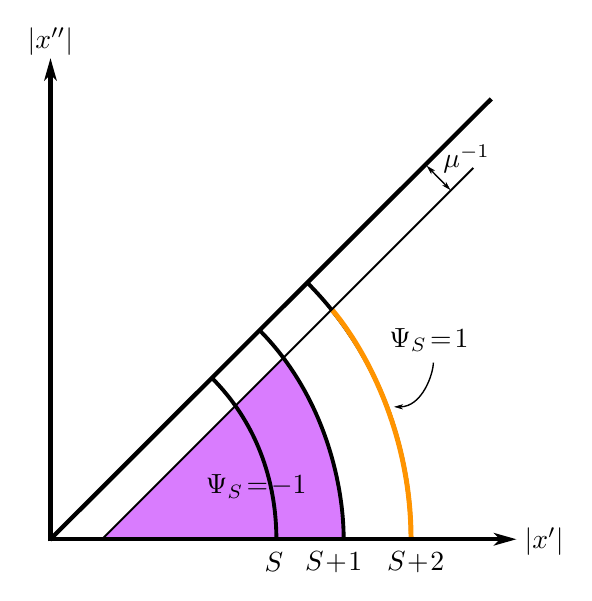
\begin{tikzpicture}[y=0.80pt, x=0.80pt, yscale=-1.000000, xscale=1.000000, inner sep=0pt, outer sep=0pt]


%region-down
\path[scale=0.938,fill=lila_custom, opacity = 0.7, line width=0.400pt] (248.0459,242.6193) ..
controls (275.7060,284.1286) and (276.2013,310.5581) .. (276.7985,330.5197) ..
controls (233.8448,330.5197) and (216.3370,330.5469) .. (160.2334,330.5469) ..
controls (186.2822,304.6380) and (219.4410,271.2569) .. (248.0459,242.6193) --
cycle;



%big circle
\path[draw=black,line join=miter,line cap=butt,line width=1.4pt]
(243.0000,193.8560) .. controls (275.7522,226.7370) and (289.9164,269.7115) ..
(289.9164,309.8622);

%big circle2
\path[draw=naranja_custom,line join=miter,line cap=butt,line width=1.8pt]
(243.0000+11,193.8560+12) .. controls (275.7522-9,226.7370-6) and (289.9164,258.7115) ..
(289.9164,309.8622);

%x-axis    
\path[draw=black,line join=miter,line cap=butt,line width=1.5pt]
(126.5055,309.8063) -- (330.4872,309.8063);

%x-axis cap    
\path[draw=black,fill=black,even odd rule,line width=0.497pt]
(330.4872,309.8063) -- (328.1493,312.1289) -- (336.3320,309.8063) --
(328.1493,307.4838) -- cycle;

%y-axis
\path[draw=black,line join=miter,line cap=butt,line width=1.5pt]
(127.0562,310.75) -- (127.0562,99.5223);

%y-axis cap    
\path[draw=black,fill=black,even odd rule,line width=0.497pt] (127.0562,99.5223)
-- (129.3788,101.8602) -- (127.0562,93.6775) -- (124.7336,101.8602) -- cycle;



%medium circle
\path[draw=black,line join=miter,line cap=butt,line width=1.4pt]
(221.4938,215.3997) .. controls (250.7785,244.9692) and (259.4986,284.9193) ..
(259.4986,309.8622);

%small circle    
\path[draw=black,line join=miter,line cap=butt,line width=1.4pt]
(199.9500,236.9435) .. controls (222.0483,259.0975) and (229.1002,286.5606) ..
(229.1002,309.8622);

%cone   
\path[draw=black,line join=miter,line cap=butt,miter limit=4.00,even odd
rule,line width=1.57pt] (126.7629,310.0643) -- (326.1869,110.8844);

%cone+1    
\path[draw=black,line join=miter,line cap=butt,even odd rule,line width=0.704pt]
(150.2563,309.8481) -- (318.0555,142.0518);

%cone-1 
%\path[draw=black,line join=miter,line cap=butt,even odd rule,line width=0.704pt]
%(127.1847,287.2416) -- (299.4946,114.9526); 


%Linea Cota
\path[draw=black,line join=miter,line cap=butt,line width=0.5pt]
(298.3343,142.4919) -- (306.3936,150.7321);


%Flecha Izquierda Cota
\path[draw=black,fill=black,even odd rule,line width=0.200pt]
(298.9657,143.1375) -- (300.2914,143.1522) -- (297.3269,141.4619) --
(298.9510,144.4632) -- cycle;

%Flecha Derecha Cota
\path[draw=black,fill=black,even odd rule,line width=0.200pt]
(305.7622,150.0865) -- (304.4364,150.0718) -- (307.4010,151.7621) --
(305.7769,148.7608) -- cycle;

%Cota naranja
\path[draw=black,line join=miter,line cap=butt,line width=0.5pt]
(300, 230) .. controls (300, 235) and (295, 250) ..
(285, 250);

%Flecha cota naranja
\path[draw=black,fill=black,even odd rule,line width=0.200pt]
(285, 250) -- (285+0.9375, 250+0.9375) -- (285-2.3437, 250) --
(285+0.9375, 250-0.9375) -- cycle;

\node at (315,138) {\normalsize $\mu^{-1}$};
\node at (127,85) {\normalsize $|x''|$};
\node at (350, 311) {\normalsize $|x'|$};
\node at (228,320) {\normalsize $S$};
\node at (255, 320) {\normalsize $S\!+\!1$};
\node at (292, 320) {\normalsize $S\!+\!2$};
\node at (334, 101) {\normalsize $\ccal$};
\node at (298, 220) {\normalsize $\Psi_S\! = \!1$};
\node at (220, 286) {\normalsize $\Psi_S\! = \!-1$};


\end{tikzpicture}


	\end{subfigure}
	\hspace{0.28\textwidth}
	\begin{subfigure}{0.21\textwidth}
		\centering
		\definecolor{azul_custom}{RGB}{66,240,209}
\definecolor{lila_custom}{RGB}{201,69,254}
\definecolor{naranja_custom}{RGB}{255,148,0}


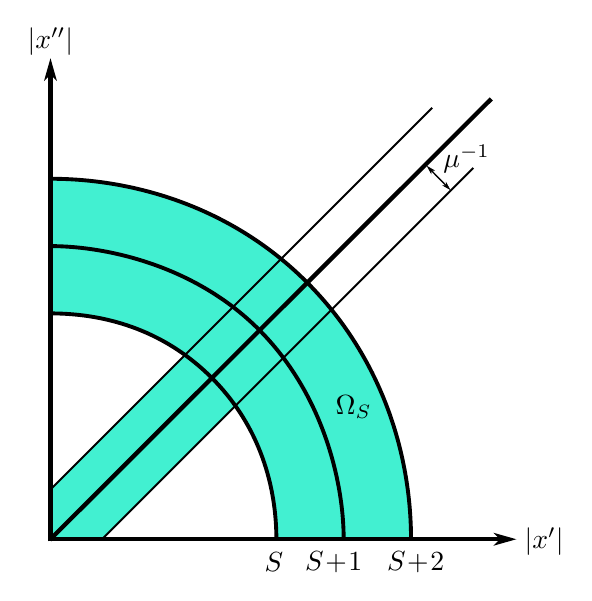
\begin{tikzpicture}[y=0.80pt, x=0.80pt, yscale=-1.000000, xscale=1.000000, inner sep=0pt, outer sep=0pt]


%region
\path[fill=azul_custom,line cap=round,miter limit=4.00,line width=1.216pt]
(210.3958,249.7906) .. controls (188.0101,272.1763) and (172.1936,287.9233) ..
(150.1544,309.9625) .. controls (148.2221,309.9625) and (137.7690,309.7049) ..
(127.0089,309.7371) .. controls (127.0089,300.7477) and (127.0826,301.1491) ..
(127.0826,287.3606) .. controls (136.2973,278.1061) and (177.3049,237.1011) ..
(187.7910,226.5786) .. controls (170.0299,214.0930) and (149.7638,207.7938) ..
(127.0312,207.7938) .. controls (127.0312,190.9391) and (126.9993,161.0751) ..
(126.9993,146.8284) .. controls (170.9394,146.8284) and (208.6039,162.4681) ..
(243.0000,193.8560) .. controls (271.9385,225.9716) and (289.9164,263.3638) ..
(289.9164,309.8622) .. controls (260.7310,309.8622) and (257.9656,309.8622) ..
(229.1006,309.8622) .. controls (229.1006,279.3951) and (221.7362,269.4328) ..
(210.3958,249.7907) -- cycle;


%x-axis    
\path[draw=black,line join=miter,line cap=butt,line width=1.5pt]
(126.5055,309.8063) -- (330.4872,309.8063);

%x-axis cap    
\path[draw=black,fill=black,even odd rule,line width=0.497pt]
(330.4872,309.8063) -- (328.1493,312.1289) -- (336.3320,309.8063) --
(328.1493,307.4838) -- cycle;

%y-axis
\path[draw=black,line join=miter,line cap=butt,line width=1.5pt]
(127.0562,310.75) -- (127.0562,99.5223);

%y-axis cap    
\path[draw=black,fill=black,even odd rule,line width=0.497pt] (127.0562,99.5223)
-- (129.3788,101.8602) -- (127.0562,93.6775) -- (124.7336,101.8602) -- cycle;


%big circle
\path[draw=black,line join=miter,line cap=butt,line width=1.4pt]
(127.0312,146.9770) .. controls (166.9982,146.9770) and (210.2478,160.9750) ..
(243.0000,193.8560) .. controls (275.7522,226.7370) and (289.9164,269.7115) ..
(289.9164,309.8622);

%medium circle
\path[draw=black,line join=miter,line cap=butt,line width=1.4pt]
(127.0312,177.3949) .. controls (151.7088,177.3949) and (192.2090,185.8302) ..
(221.4938,215.3997) .. controls (250.7785,244.9692) and (259.4986,284.9193) ..
(259.4986,309.8622);

%small circle    
\path[draw=black,line join=miter,line cap=butt,line width=1.4pt]
(127.0312,207.7933) .. controls (150.2506,207.7933) and (177.3815,214.3180) ..
(199.9500,236.9435) .. controls (222.0483,259.0975) and (229.1002,286.5606) ..
(229.1002,309.8622);

%cone   
\path[draw=black,line join=miter,line cap=butt,miter limit=4.00,even odd
rule,line width=1.57pt] (126.7629,310.0643) -- (326.1869,110.8844);

%cone+1    
\path[draw=black,line join=miter,line cap=butt,even odd rule,line width=0.704pt]
(150.2563,309.8481) -- (318.0555,142.0518);

%cone-1 
\path[draw=black,line join=miter,line cap=butt,even odd rule,line width=0.704pt]
(127.1847,287.2416) -- (299.4946,114.9526); 

%Linea Cota
\path[draw=black,line join=miter,line cap=butt,line width=0.5pt]
(298.3343,142.4919) -- (306.3936,150.7321);


%Flecha Izquierda Cota
\path[draw=black,fill=black,even odd rule,line width=0.200pt]
(298.9657,143.1375) -- (300.2914,143.1522) -- (297.3269,141.4619) --
(298.9510,144.4632) -- cycle;

%Flecha Derecha Cota
\path[draw=black,fill=black,even odd rule,line width=0.200pt]
(305.7622,150.0865) -- (304.4364,150.0718) -- (307.4010,151.7621) --
(305.7769,148.7608) -- cycle;

\node at (315,138) {\normalsize $\mu^{-1}$};
\node at (127,85) {\normalsize $|x''|$};
\node at (350, 311) {\normalsize $|x'|$};
\node at (228,320) {\normalsize $S$};
\node at (255, 320) {\normalsize $S\!+\!1$};
\node at (292, 320) {\normalsize $S\!+\!2$};
\node at (334, 101) {\normalsize $\ccal$};
\node at (264, 250) {\normalsize $\Omega_S$};

\end{tikzpicture}











	\end{subfigure}
	\caption{(a) The $1$ and $-1$ level sets of $\Psi_S$. (b) The set $\Omega_S$.}
	\label{Fig:PsiSandOmegaS}
\end{figure}

The set $\Omega_S$ is the preimage of $1$ through $d_S$ in $\overline{B_{S+2}}$ ---see Figure~\ref{Fig:PsiSandOmegaS}~(b). Furthermore, it is easy to see that its measure is of order $2m-1$. That is,
\begin{equation}
\label{Eq:MeasureOmegaS}
|\Omega_S| \leq C\,S^{2m-1},
\end{equation}
with a constant $C$ depending only on $m$ and $\mu$. To see this, follow the computations in the proof of the energy estimate for the local equation in Theorem~1.3 of \cite{CabreTerraI}.


Now we show some auxiliary results concerning the previous definitions, needed in the proof of Theorem~\ref{Th:EnergyEstimate}.

\begin{lemma}
\label{Lemma:AdaptedLipschitzConditionWith_dFunction}
Given $S>0$, if either $(x,y) \in \left(\Omega_S\cap \ocal\right) \times \ical$ or $(x,y)\in \left(B_{S+2}\cap \ocal\right) \times \ocal$, then
$$ 
|\Psi_S(x) - \Psi_S(y)| \leq C \frac{|x-y|}{d_S(x)} \ \ \ \ \ \textrm{whenever} \ \ |x-y|\leq d_S(x), 
$$
with $C>0$ depending only on $m$ and $\mu$, and thus independent of $S$.
\end{lemma}

\begin{proof}
First, note that if $x\in \Omega_S$, then $d_S(x)=1$ and $x,y\in B_{S+3}$ whenever $|x-y|\leq d_S(x)=1$. Therefore, the result follows from the Lipschitz continuity of $\Psi_S$ in $B_{S+3}$. Hence, we only need to establish the result for the case $x\in B_S\cap \{\mu \dist(\cdot,\ccal)> 1\} \cap \ocal$ and $y\in \ocal$. Under these assumptions, we have that $\Psi_S(x)=-1$ (see Figure~\ref{Fig:PsiSandOmegaS}) and $d_S(x) = \min\{S+1-|x|,\mu \dist(x,\ccal)\} \leq S+1-|x|$. Thus, if $|x-y|\leq d_S(x)$, it holds
$$
 |y|\leq |x-y| + |x| \leq d_S(x)+|x| \leq S+1. 
$$

Therefore, we have to show
\begin{equation}
\label{Eq:TriangularIneqProof1}
	|1+\Psi_S(y)|\leq C\dfrac{|x-y|}{\min\{S+1-|x|,\mu \dist(x,\ccal)\}}
\end{equation}
for $x\in B_S\cap \{\mu\dist(x,\ccal)>1\} \cap \ocal$ and $y \in B_{S+1}\cap \ocal$.

Now we distinguish two cases: either $\mu\dist(y,\ccal)\geq 1$ or $\mu \dist(y,\ccal)< 1$. Assume first that $y\in B_{S+1} \cap \{\mu \dist(\cdot,\ccal)\geq 1\}\cap \ocal$. Then, $\Psi_S(y)=-1$ and \eqref{Eq:TriangularIneqProof1} is trivial. Hence, it only remains to show \eqref{Eq:TriangularIneqProof1} in the case $y\in B_{S+1} \cap \{\mu \dist(\cdot,\ccal) < 1\}\cap \ocal$. Note that under these assumptions, $\Psi_S(x)=-1$ and $\Psi_S(y)=-\mu \dist(y,\ccal)$. 

We claim that for $x \in \{\mu \dist(\cdot,\ccal)\geq 1\}$ and $y \in \{\mu \dist(\cdot,\ccal)\leq 1\}$ it holds
\begin{equation}
\label{Eq:TriangularIneqProof2}
|1-\mu \dist(y,\ccal)|\leq \dfrac{|x-y|}{\dist(x,\ccal)}\,.
\end{equation}
Assuming this claim to be true, we have that if $x\in B_S\cap \{\mu \dist(x,\ccal)\geq 1\} \cap \ocal$ and $y\in B_{S+1} \cap \{\mu \dist(\cdot,\ccal)\leq 1\}\cap \ocal$, then
$$ 
|\Psi_S(x)-\Psi_S(y)| = |1-\mu \dist(y,\ccal)| \leq \frac{|x-y|}{\dist(x,\ccal)} \leq  \mu \frac{|x-y|}{d_S(x)},
$$
completing the proof.

Let us show now \eqref{Eq:TriangularIneqProof2}. Given $x,y \in \R^{2m}$ it is easy to prove by using the triangular inequality and the definition of distance to the cone that
\begin{equation} 
\label{Eq:TriangularCone}
\dist(x,\ccal) \leq |x-y| + \dist(y,\ccal).
\end{equation}
Therefore, since $\mu \dist(x,\ccal)\geq 1$, we have
\begin{equation} 
\label{Eq:TriangularCone2}
1-\mu |x-y|- \mu \dist(y,\ccal) \leq 1-\mu\dist(x,\ccal) \leq 0
\end{equation}
Now, multiplying \eqref{Eq:TriangularCone} by $|1-\mu\dist(y,\ccal)|$, and using that $\mu \dist(y,\ccal)\leq 1$ and \eqref{Eq:TriangularCone2}, we obtain
\begin{align*}
|1-\mu\dist(y,\ccal)|\,\dist(x,\ccal) &\leq (1-\mu\dist(y,\ccal)) \left(|x-y| + \dist(y,\ccal)\right) \\
&= |x-y|+\dist(y,\ccal) \left\{ 1 -\mu |x-y|- \mu \dist(y,\ccal) \right\} \\
&\leq |x-y|.
\end{align*}
\end{proof}

Another auxiliary result that we will need in the proof of Theorem~\ref{Th:EnergyEstimate} is the following estimate for the function $d_S$. 

\begin{lemma}
\label{Lemma:Integrability_dFunction}
Given $\s \in (0,1)$ and $B_{S+2}\subset \R^{2m}$ with $S>2$, we have
$$ \int_{B_{S+2}} d_S(x)^{-2\s} \d x \leq \begin{cases}
C \ S^{2m-2\s}\ \ \ \ &\textrm{if } \ \ \s\in(0,1/2),\\
C\ \log(S)\,S^{2m-1}\ \ \ \ &\textrm{if } \ \ \s=1/2,\\
C \ S^{2m-1}\ \ \ \ &\textrm{if } \ \ \s\in(1/2,1),\\
\end{cases} $$
with $C>0$ independent of $S$ and depending only on $m$, $\s$, and $\mu$.
\end{lemma}


\begin{proof}
In order to prove this result we first note that $d_S(x)=1$ in $\Omega_S$. Thus, the contribution to the integral of this part is just the measure of the set $\Omega_S$ ---see \eqref{Eq:MeasureOmegaS}. That is,
$$
\int_{\Omega_S} d_S(x)^{-2\s} \d x = |\Omega_S| \leq C\,S^{2m-1}.
$$
Since $S>2$, the desired estimate for this integral follows straightforward.

For the other part of the integral we can write
\begin{align*}
\int_{B_{S+2}\setminus \Omega_S} d_S(x)^{-2\s} \d x &= \int_{B_{S}\cap \{\mu \dist(x,\ccal)>1\}} d_S(x)^{-2\s} \d x \\
& \leq \int_{B_{S}\cap \{\mu \dist(x,\ccal)>1\}} \left( S+1-|x| \right)^{-2\s} \d x \\
& \quad \quad + \int_{B_{S}\cap \{\mu \dist(x,\ccal)>1\}} \dist(x,\ccal)^{-2\s} \d x.
\end{align*}
The desired estimate for the first integral can be found in \cite{SavinValdinoci-EnergyEstimate}. Therefore, in order to complete the proof, it only remains to estimate the second integral. This can be done by writing it in $(\euscr{y},\euscr{z})$ variables, where
%\todo{elegir fuente}
$$
\euscr{y} := \dfrac{|x'|+|x''|}{\sqrt{2}} \, \quad \text{ and } \euscr{z} := \dfrac{|x'|-|x''|}{\sqrt{2}}\,.
$$
Note that $\euscr{z}$ is the signed distance to the cone (see Lemma~4.2 in \cite{CabreTerraI}). Thus,
\begin{align*}
\int_{B_{S}\cap \{\mu \dist(x,\ccal)>1\}} \dist(x,\ccal)^{-2\s} \d x &\leq C \int \int_{B_{S}\cap \{\euscr{y}\geq|\euscr{z}|>1/\mu\}} |\euscr{z}|^{-2\s} \, (\euscr{y}^2-\euscr{z}^2)^{m-1} \d \euscr{y}\d \euscr{z} \\
& \leq C \int \int_{B_{S}\cap \{\euscr{y}\geq|\euscr{z}|>1/\mu\}} |\euscr{z}|^{-2\s} \, \euscr{y}^{2m-2} \d \euscr{y}\d \euscr{z} \\
& \leq C\, \int_{1/\mu}^S \d \euscr{z}   \ \euscr{z}^{-2\s}\int_0^S \d \euscr{y}\  \euscr{y}^{2m-2} \\
& \leq \begin{cases}
C \ S^{2m-2\s}\ \ \ \ &\textrm{if } \ \ \s\in(0,1/2),\\
C\ \log(S)\,S^{2m-1}\ \ \ \ &\textrm{if } \ \ \s=1/2,\\
C \ S^{2m-1}\ \ \ \ &\textrm{if } \ \ \s\in(1/2,1).\\
\end{cases}
\end{align*}
\end{proof}

Note that the $(\euscr{y},\euscr{z})$ variables used in the previous computation are usually very helpful when dealing with doubly radial odd functions ---see \cite{CabreTerraI, CabreTerraII, Cabre-Saddle, Cinti-Saddle,Cinti-Saddle2, Felipe-Sanz-Perela:SaddleFractional}.

The last auxiliary result we need in order to establish the energy estimate is the following inequality.

\begin{lemma}
\label{Lemma:InteractionInequalityMinimumFunction}
Let $\rho>0$ and let $A\subset B_\rho \subset \R^{2m}$ be a set of double revolution that is symmetric with respect to the Simons cone, i.e., $A^\star = A$. Let $\omega, \phi, \varphi \in \widetilde{\H}^K(B_\rho)$, with $K$ radially symmetric, be such that
\begin{equation}
	\label{Eq:InteractionMinHyp}
	\begin{cases}
	\omega = \phi \leq \varphi \ \ \ \ \textrm{in } \ \ \ \ocal \setminus A\,,\\
	\omega = \varphi \leq \phi \ \ \ \ \textrm{in } \ \ \ A \cap \ocal\,.
	\end{cases}
\end{equation}
Then, if $K$ satisfies \eqref{Eq:KernelInequality}, it holds
\begin{align*}
I_\omega(A \cap \ocal, \ocal \setminus A) \leq I_\phi(A \cap \ocal, \ocal \setminus A) + I_\varphi(A \cap \ocal, \ocal \setminus A)\,,
\end{align*}
where $I_w(\cdot, \cdot)$ is the interaction defined in \eqref{Eq:DefIw}.
\end{lemma}

\begin{proof}
A simple computation shows that if $x\in A \cap \ocal $ and $y\in \ocal \setminus A$ we have that
$$ |\phi(x)-\phi(y)|^2+|\varphi(x)-\varphi(y)|^2\geq |\omega(x)-\omega(y)|^2. $$
Indeed, using \eqref{Eq:InteractionMinHyp} we see that
\begin{align*}
|\phi(x)-\phi(y)|^2+|\varphi(x)&-\varphi(y)|^2 - |\omega(x)-\omega(y)|^2 \\
&= |\phi(x)-\phi(y)|^2+|\varphi(x)-\varphi(y)|^2 - |\varphi(x)-\phi(y)|^2 \\
&= \phi^2(x)-2\phi(x)\phi(y)+\varphi^2(y)-2\varphi(x)\varphi(y)+2\varphi(x)\phi(y) \\
&= \left( \phi(x) - \varphi(y)\right) ^2+2\left( \phi(x)-\varphi(x) \right) \left( \varphi(y)-\phi(y) \right) \\
&\geq 0.
\end{align*}
Therefore, by using this inequality and the reflexion property of the kernel, \eqref{Eq:KernelInequality}, we obtain
\begin{align*}
I_\phi(A \cap \ocal, \ocal \setminus A) &+ I_\varphi(A \cap \ocal, \ocal \setminus A) - I_\omega(A \cap \ocal, \ocal \setminus A) =\\
&\hspace{-26mm}= \int_{A \cap \ocal} \! \d x \int_{\ocal\setminus A} \! \d y \, \Big( 4\left\{\phi^2(x)+\phi^2(y)+\varphi^2(x)+\varphi^2(y)-\omega^2(x)-\omega^2(y) \right\} \overline{K}(x,y^\star) \Big.\\
&\hspace{-18mm}\Big.+  2\left\{|\phi(x)-\phi(y)|^2+|\varphi(x)-\varphi(y)|^2-|\omega(x)-\omega(y)|^2 \right\} \left\{\overline{K}(x,y)-\overline{K}(x,y^\star)\right\}\Big)\\
&\hspace{-26mm}\geq 4\int_{A \cap \ocal} \! \d x \int_{\ocal\setminus A} \! \d y \, \left\{ \phi^2(x)+\varphi^2(y)\right\} \overline{K}(x,y^\star) \geq 0.
\end{align*}
\end{proof}



With all these ingredients we can establish now the desired energy estimate.

\begin{proof}[Proof of Theorem~\ref{Th:EnergyEstimate}]

Note that since $u$ is a minimizer of $\ecal$ in $B_R$, by Lemma~\ref{Lemma:DecreaseEnergy} we can assume without loss of generality that $-1 \leq u \leq 1$, $u \geq 0$ in $\ocal$, and $u \leq 0$ in $\ical$. 

\textbf{Step 1. We show that $0\leq u < 1$ in $\ocal$.} 

In order to prove it, we first show that $u$ is a classical solution to
\begin{equation}
\label{Eq:ProofEnergyEstimateProblemBR}
	\beqc{\PDEsystem}
	L_K  u &=& f(u) & \textrm{ in } B_R\,,\\
	u &=& 0 & \textrm{ in }\R^{2m} \setminus B_R.
	\eeqc
\end{equation}
To see this, we consider perturbations $u +  \varepsilon \xi$ with $\varepsilon>0$. On the one hand, take $\xi \in \widetilde{\H}^K_{0, \,\mathrm{odd}}(B_R)$. Then, since $u$ is a minimizer among functions in $\widetilde{\H}^K_{0, \,\mathrm{odd}}(B_R)$, we get
$$
0 = \dfrac{\d}{\d \varepsilon}\evalat{\varepsilon = 0} \ecal(u +  \varepsilon \xi, B_R) = \langle u,\xi \rangle_{\widetilde{\H}^K_0(B_R)} - \langle f(u),\xi \rangle_{L^2(B_R)}\,.
$$
On the other hand, take $\xi \in \widetilde{\H}^K_{0, \,\mathrm{even}}(B_R)$. Since $u$ is odd with respect to the Simons cone, the same holds for $f(u)$ ---recall that $f$ is odd. Then, by Remark~\ref{Remark:DecompositionHK} we find that
$$
\langle u,\xi \rangle_{\widetilde{\H}^K_0(B_R)} = 0 \quad \textrm{ and } \quad  \langle f(u),\xi \rangle_{L^2(B_R)} = 0\,.
$$
Therefore, 
$$
\langle u,\xi \rangle_{\widetilde{\H}^K_0(B_R)} = \langle f(u),\xi \rangle_{L^2(B_R)}
$$
for every $\xi \in\widetilde{\H}^K_0(B_R)$ with compact support in  $B_R$. By approximation, $\xi$ can be taken to be $C^\infty_c(B_R)$. Thus,
$$
\int_{\R^{2m}}\int_{\R^{2m}} \{u(x)-u(y)\}\{\xi(x)-\xi(y)\} K(|x-y|) \d x \d y = \int_{\R^{2m}} f(u(x)) \xi(x) \d x
$$
for every $\xi \in C^\infty_c(\Omega)$ that is doubly radial. Finally, by Proposition~\ref{Prop:WeakSolutionForAllTestFunctions}, $u$ is a weak solution to \eqref{Eq:ProofEnergyEstimateProblemBR}, and in view of the regularity theory for operators in $\lcal_0$ (see Remark~\ref{Remark:InteriorRegularity}), since $u$ is bounded, it is a classical solution.

Since $u$ is a classical solution that is odd and continuous, it follows that $u \not \equiv 1$ in $\ocal$. Therefore, by the usual strong maximum principle (recall that $u\leq 1$), we get $0\leq u < 1$ in $\ocal$. 

\textbf{Step 2. We build a suitable competitor for $u$ and compare their energies.}

For $x\in \overline{\ocal}$ we define
$$ 
v(x) := \min\{u(x),\Psi_S(x)\}, 
$$
and we define it in $\ical$ by considering its odd reflection with respect to the Simons cone. Recall that $\Psi_S$ is defined in \eqref{Eq:DefPsiS} and it is zero on the cone $\ccal$. Let us also define
$$
A :=(\{\Psi_S < u\}\cap \ocal) \cup (\{\Psi_S < u\}\cap \ocal)^\star. 
$$
Thus, $v = \Psi_S < u$ in $A\cap \ocal$ and $v=u\leq\Psi_S$ in $\ocal \setminus A$. 

We claim that if we take
\begin{equation}
	\label{Eq:ChoiceMu}
	\mu = \norm{u}_{\mathrm{Lip}(\overline{B_{S+4}})},
\end{equation}
we have the inclusions
\begin{equation}
\label{Eq:EnergyEstimateProofInclusionsA}
	B_{S+1}\setminus \ccal \subset A \subset B_{S+2}\,.
\end{equation}
Let us show this. Note first that by symmetry and the fact that $\Psi_S = u =0$ in $\ccal$, we only need to prove that 
$$
	B_{S+1} \cap \ocal\subset A \cap \ocal\subset B_{S+2}\cap \ocal\,.
$$
On the one hand, if $ x\in B_{S+1}\cap \ocal$, then $\Psi_S(x) = -\min\{1,\mu\dist(x,\ccal)\} < 0 \leq u(x)$. Thus, $x\in A\cap \ocal$. On the other hand, if $ x\in A\cap \ocal$ then $\Psi_S(x) < u(x) < 1$ and this can only happen if $x\in B_{S+2}\cap \ocal$. Let us show this. First, note that $\Psi_S \equiv 1$ in $\ocal\setminus B_{S+4}$ and in $(B_{S+4}\setminus B_{S+2})\cap \{\mu \dist(\cdot, \ccal)\geq 1\} \cap \ocal$ ---see Figure~\ref{Fig:PsiSandOmegaS} (a). Therefore, we only need to see that 
$$
u(x) \leq \Psi(x) = \mu \dist (x,\ccal) \quad \text{ for every } x \in (B_{S+4}\setminus B_{S+2})\cap \{\mu \dist(\cdot, \ccal)< 1\} \cap \ocal.
$$
By the choice of $\mu$ in \eqref{Eq:ChoiceMu}, we know that
$$
|u(x) - u(y)|\leq \mu |x-y| \quad \text{ for every } x, \ y \in \overline{B_{S+4}}.
$$
Thus, by taking $x \in (B_{S+4}\setminus B_{S+2})\cap \{\mu \dist(\cdot, \ccal)< 1\} \cap \ocal$ and  $y\in \ccal$ to be a point realizing $\dist(x,\ccal)$, we obtain the desired inequality, concluding the proof of \eqref{Eq:EnergyEstimateProofInclusionsA}. Note that if $x\in \overline{B_{S+4}}$, it is easy to check that $y\in \overline{B_{S+4}}$.

By \eqref{Eq:EnergyEstimateProofInclusionsA}, both $u$ and $v$ are equal outside $B_{S+2} \subset B_R$, and therefore $v$ is an admissible competitor. Comparing the energies of $u$ and $v$ we will obtain the desired estimate. 

Using the expression \eqref{Eq:ShortExpressionEnergy}, let us decompose the energy of $u$ in $B_R$ in the following way:
\begin{align*}
\ecal(u,B_R) &= \frac{1}{4}I_u(A \cap \ocal, A \cap \ocal) + \frac{1}{2}I_u(A \cap \ocal, \ocal \setminus A) \\
& \hspace{5mm} + \frac{1}{4}I_u\big((\ocal \setminus A) \cap B_R, (\ocal \setminus A) \cap B_R\big) + \frac{1}{2}I_u\big((\ocal \setminus A) \cap B_R, \ocal \setminus B_R\big) \\
& \hspace{5mm} + \int_A G(u) \d x + \int_{B_R\setminus A} G(u) \d x
\end{align*}
Since $u$ is a minimizer, $v=\Psi_S$ in $A\cap \ocal$, and $u=v$ in $\ocal\setminus A$,  from the previous expression we obtain
\begin{align*}
0 &\leq \ecal(v,B_R)-\ecal(u,B_R) = \frac{1}{4}I_{\Psi_S}(A \cap \ocal, A \cap \ocal) - \frac{1}{4}I_u(A \cap \ocal, A \cap \ocal)\\
& \hspace{5mm} +  \frac{1}{2} I_v(A \cap \ocal, \ocal \setminus A) -  \frac{1}{2} I_u(A \cap \ocal, \ocal \setminus A) + \int_A G(\Psi_S) \d x - \int_{A} G(u) \d x.
\end{align*}

Now, recalling that $v = \min\{u,\Psi_S\}$ in $\ocal$, we can apply Lemma \ref{Lemma:InteractionInequalityMinimumFunction} with $\omega = v$, $\Psi_S = \varphi$, and $u= \phi$, to get $I_v(A \cap \ocal, \ocal\setminus A) \leq I_u(A \cap \ocal, \ocal\setminus A) + I_{\Psi_S}(A \cap \ocal, \ocal\setminus A)$. Therefore,
\begin{align*}
\frac{1}{4}I_u(A \cap \ocal, A \cap \ocal) + \int_{A} G(u) \d x &\leq \frac{1}{4}I_{\Psi_S}(A \cap \ocal, A \cap \ocal) +  \frac{1}{2} I_{\Psi_S}(A \cap \ocal, \ocal \setminus A) \\
& \quad \quad  + \int_A G(\Psi_S)  \d x \\
&= \ecal(\Psi_S, A) \leq \ecal(\Psi_S,B_{S+2}).
\end{align*}
From this and using the inclusions of \eqref{Eq:EnergyEstimateProofInclusionsA}, we deduce an estimate for the energy of $u$ in $B_S$ as follows.
\begin{align*}
\ecal(u,B_S) &\leq \frac{1}{4}I_u(A \cap \ocal, A \cap \ocal) + \int_{A} G(u) \d x +  \frac{1}{2} I_u(B_S \cap \ocal, \ocal \setminus B_{S+1}) \\
& \leq  \ecal(\Psi_S,B_{S+2}) +  \frac{1}{2} I_u(B_S \cap \ocal, \ocal \setminus B_{S+1}).
\end{align*}
Thus, to obtain the desired energy estimate we only have to bound the right-hand side of the last inequality.


\textbf{Step 3. We estimate the remaining terms.}

In the following arguments, we use the definition of the energy that involves the original kernel $K$ and not $\overline{K}$. Moreover, the letter $C$ will denote different constants depending on $m$, $\s$, $\mu$, $G$, and $\Lambda$.

\textbf{3.1. Estimate for $\ecal(\Psi_S,B_{S+2})$.}
First, by using the change of variables given by $(\cdot)^\star$ and the ellipticity of $K$ ---that is, condition \eqref{Eq:Ellipticity}---, we obtain
\begin{align*}
\ecal(\Psi_S,B_{S+2}) &= \frac{1}{4} \int_{B_{S+2}} \d x \int_{B_{S+2}} \d y\ |\Psi_S(x)-\Psi_S(y)|^2K(|x-y|)  \\
&\hspace{5mm} +\frac{1}{2} \int_{B_{S+2}} \d x \int_{\R^{2m} \setminus B_{S+2}} \d y \ |\Psi_S(x)-\Psi_S(y)|^2K(|x-y|) \\
&\hspace{5mm} + \int_{B_{S+2}} G(\Psi_S)  \d x\\
&\leq \frac{1}{2} \int_{B_{S+2}} \d x \int_{\R^{2m}} \d y\ |\Psi_S(x)-\Psi_S(y)|^2K(|x-y|) + \int_{B_{S+2}} G(\Psi_S) \d x \\
&= \int_{B_{S+2} \cap \ocal} \d x \int_{\R^{2m}} \d y\ |\Psi_S(x)-\Psi_S(y)|^2K(|x-y|)  + \int_{B_{S+2}} G(\Psi_S) \d x \\
&\leq \Lambda\, c_{n,\s} \int_{B_{S+2} \cap \ocal} \d x \int_{\R^{2m}} \d y \ \frac{|\Psi_S(x)-\Psi_S(y)|^2}{|x-y|^{2m+2\s}} + \int_{B_{S+2}} G(\Psi_S) \d x.
\end{align*}
Now, we split the kinetic energy into three terms. We get
\begin{align*}
\ecal(\Psi_S,B_{S+2}) &\leq \Lambda\, c_{n,\s} \int_{B_{S+2} \cap \ocal} \d x \int_{\ocal} \d y \frac{|\Psi_S(x)-\Psi_S(y)|^2}{|x-y|^{2m+2\s}} \\
&\hspace{5mm} + \Lambda\, c_{n,\s} \int_{\Omega_S \cap \ocal} \d x \int_{\ical} \d y \frac{|\Psi_S(x)-\Psi_S(y)|^2}{|x-y|^{2m+2\s}} \\
&\hspace{5mm} + \Lambda\, c_{n,\s} \int_{(B_{S+2}\setminus \Omega_S) \cap \ocal} \d x \int_{\ical} \d y \frac{|\Psi_S(x)-\Psi_S(y)|^2}{|x-y|^{2m+2\s}} + \int_{B_{S+2}} G(\Psi_S) \d x\\
&=:\Lambda\, c_{n,\s} (I_1+I_2+I_3)+I_G,
\end{align*}
where $\Omega_S$ is defined in \eqref{Eq:DefOmegaS}. 

Let us estimate these four integrals. To control $I_1$, we use Lemma~\ref{Lemma:AdaptedLipschitzConditionWith_dFunction} and the fact that $\Psi_S$ is bounded by $1$.
\begin{align*}
I_1 &= \int_{B_{S+2} \cap \ocal} \int_{\ocal} \frac{|\Psi_S(x)-\Psi_S(y)|^2}{|x-y|^{2m+2\s}} \d y\d x\\
&= \int_{B_{S+2} \cap \ocal} \int_{\ocal\cap\{|x-y|\leq d_S(x)\}} \frac{|\Psi_S(x)-\Psi_S(y)|^2}{|x-y|^{2m+2\s}} \d y\d x\\
&\hspace{5mm} + \int_{B_{S+2} \cap \ocal} \int_{\ocal\cap\{|x-y|\geq d_S(x)\}} \frac{|\Psi_S(x)-\Psi_S(y)|^2}{|x-y|^{2m+2\s}} \d y\d x\\
&\leq C \int_{B_{S+2} \cap \ocal} d_S(x)^{-2}\left(\int_{\ocal\cap\{|x-y|\leq d_S(x)\}} |x-y|^{2-2m-2\s} \d y\right)\d x\\
&\hspace{5mm} + C \int_{B_{S+2} \cap \ocal} \left(\int_{\ocal\cap\{|x-y|\geq d_S(x)\}} |x-y|^{-2m-2\s} \d y \right)\d x\\
&\leq C \int_{B_{S+2} \cap \ocal} d_S(x)^{-2}\left(\int_0^{d_S(x)} \rho^{1-2\s} \d \rho\right)\d x + C \int_{B_{S+2} \cap \ocal}  \left(\int_{d_S(x)}^\infty \rho^{-1-2\s} \d\rho\right) \d x\\
&\leq C \int_{B_{S+2} \cap \ocal} d_S(x)^{-2\s} \d x.
\end{align*}

The bound of $I_2$ is essentially the same using also Lemma~\ref{Lemma:AdaptedLipschitzConditionWith_dFunction} and the inclusion $\Omega_S \subset B_{S+2}$. That is,
\begin{align*}
I_2 &\leq C \int_{\Omega_S \cap \ocal} d_S(x)^{-2}\left(\int_0^{d_S(x)} \rho^{1-2\s} \d \rho\right)\d x + C \int_{\Omega_S \cap \ocal} \left( \int_{d_S(x)}^\infty \rho^{-1-2\s} \d\rho \right) \d x\\
&\leq C \int_{\Omega _S\cap \ocal} d_S(x)^{-2\s} \d x \leq C \int_{B_{S+2} \cap \ocal} d_S(x)^{-2\s} \d x.
\end{align*}

In the case of $I_3$, we use the fact that given $x\in (B_{S+2}\setminus \Omega_S)\cap \ocal$, then $\dist(x,\ccal)\geq d_S(x)/\mu$ and therefore, for such $x$, it holds $\ical \subset \R^{2m}\setminus B_{d_S(x)/\mu}(x)$. We obtain
\begin{align*}
I_3 &= \int_{(B_{S+2}\setminus \Omega_S) \cap \ocal} \d x \int_{\ical} \d y \ \frac{|\Psi_S(x)-\Psi_S(y)|^2}{|x-y|^{2m+2\s}} \\
&\leq C \int_{(B_{S+2}\setminus \Omega_S) \cap \ocal} \d x \int_{\R^{2m}\setminus B_{d_S(x)/\mu }(x)} \d y \ |x-y|^{-2m-2\s} \\
&\leq C \int_{B_{S+2} \cap \ocal} \left(\int_{d_S(x)/\mu}^\infty \rho^{-1-2\s} \d \rho \right)\d x \leq C \int_{B_{S+2} \cap \ocal} d_S(x)^{-2\s} \d x.
\end{align*}

Finally, we estimate $I_G$. Since $\Psi_S$ is either $1$ or $-1$ in $B_{S+2}\setminus \Omega_S$, and $G(-1)=G(1)=0$, we have
\begin{align*}
I_G = \int_{B_{S+2}} G(\Psi_S) \d x= \int_{\Omega_S} G(\Psi_S)\d x \leq C | \Omega_S| \leq C\,S^{2m-1}\,,
\end{align*}
where we have used \eqref{Eq:MeasureOmegaS}. Therefore, we obtain
\begin{align*}
\ecal(\Psi_S,B_{S+2}) &\leq C \left(\int_{B_{S+2} \cap \ocal} d_S(x)^{-2\s} \d x + S^{2m-1} \right)\leq C\left(\int_{B_{S} \cap \ocal} d_S(x)^{-2\s} \d x + S^{2m-1} \right).
\end{align*}

%%%%%%%%%

\textbf{3.2. Estimate for $I_u(B_S \cap \ocal, \ocal \setminus B_{S+1})$.} First, we claim that $|x-y|\geq d_S(x)$ whenever $x\in B_S$ and $y\in \R^{2m}\setminus B_{S+1}$. Indeed, if $x\in B_S$, then it is easy to see that $d_S(x) \leq S+1-|x|$ and therefore we have $|x-y|\geq |y|-|x|\geq |y|+d_S(x)-S-1 \geq  d_S(x)$, since $|y| \geq S+1$. Thus, using this inequality and the ellipticity of $K$, we get
\begin{align*}
I_u(B_S \cap \ocal, \ocal \setminus B_{S+1}) &\leq C \int_{B_S \cap \ocal} \d x \int_{\R^{2m}\setminus B_{S+1}} \d y \ \frac{|u(x)-u(y)|^2}{|x-y|^{2m+2\s}} \\
& \leq C \int_{B_S \cap \ocal} \d x \int_{|x-y|\geq d_S(x)} \d y \ |x-y|^{-2m-2\s} \\
&\leq C \int_{B_S \cap \ocal} d_S(x)^{-2\s} \d x.
\end{align*}

\textbf{Step 4. Conclusion.}

Finally, by adding up the estimates of Step~3 and applying Lemma~\ref{Lemma:Integrability_dFunction}, we obtain the desired result. That is,
\begin{align*}
\ecal(u,B_S) &\leq \ecal(\Psi_S,B_{S+2}) +  \frac{1}{2}I_u(B_S \cap \ocal, \ocal \setminus B_{S+1}) \leq C\left(\int_{B_S \cap \ocal} d_S(x)^{-2\s} \d x + S^{2m-1} \right)\\
&\leq \begin{cases}
C \ S^{2m-2\s}\ \ \ &\textrm{if } \ \ \s\in(0,1/2),\\
C\ \log(S)\,S^{2m-1}\ \ \ \ &\textrm{if } \ \ \s=1/2,\\
C \ S^{2m-1}\ \ \ \ &\textrm{if } \ \ \s\in(1/2,1),\\
\end{cases}
\end{align*}
with a constant $C$ depending only on $m$, $\s$, $\mu$, $G$, and $\Lambda$. 

To conclude, it remains to show that $\mu$ can be controlled by a constant that depends only on $m$, $\s$, $\lambda$, $\Lambda$, and $f$ (and thus, independent of $R$ and $S$). Indeed, by Step~1, we know that $u$ solves $L_K u = f(u)$ in $B_R$ with $R> S+5$. Therefore, by applying repeatedly the estimates \eqref{Eq:C2sEstimateBalls} and \eqref{Eq:Calpha->Calpha+2sEstimateBalls} in balls centered at points of $B_{S+4}$, it is easy to see that
$$
\mu = \norm{u}_{\mathrm{Lip}(\overline{B_{S+4}})} \leq C,
$$ 
with a constant $C$ depending only on $m$, $\s$, $\lambda$, $\Lambda$, and $\norm{f}_{C^1([-1,1])}$.
\end{proof}
